\chapter{System Overview and Data Pipeline}
\label{chap:pipeline}

This chapter describes the end-to-end pipeline that turns raw Indian court-judgment text into a labelled, leakage-audited, heterogeneous knowledge graph ready for GNN training. The design reflects three constraints: (i) the corpus is large and noisy, so every stage is batch with explicit caching and auditing; (ii) the signals a predictor would want (decisions, dispositions, operative paragraphs) are precisely what a legally honest experiment must remove, so leakage prevention is baked in; and (iii) the downstream target is a graph, so text extraction and entity resolution must yield outputs reifiable as typed nodes and edges.

\section{System Architecture Overview}

The system is a six-stage pipeline. Each stage is independently re-runnable; intermediate artefacts are cached on disk so that an expensive step (OpenNyAI NER on tens of thousands of judgments, or \texttt{bge-m3} embedding on millions of text spans) is not repeated when a later stage changes.

\begin{figure}[H]
  \centering
  \begin{tikzpicture}[
      node distance=0.45cm and 0.7cm,
      every node/.style={font=\small},
      stage/.style={rectangle, rounded corners, draw=black!70, thick,
        fill=blue!6, minimum width=4.2cm, minimum height=0.95cm,
        align=center, text width=4.1cm},
      artefact/.style={rectangle, draw=black!40, dashed, fill=gray!4,
        minimum width=4.2cm, minimum height=0.7cm, align=center,
        text width=4.1cm, font=\footnotesize\itshape},
      arrow/.style={-{Stealth[length=2mm]}, thick}
    ]
    \node[stage] (s1) {\textbf{1. Document Collection}\\raw judgment
      \texttt{.txt} files};
    \node[artefact, below=of s1] (a1) {per-bucket raw corpora
      (5 legal domains)};
    \node[stage, below=of a1] (s2) {\textbf{2. OpenNyAI NER + RR}\\
      Legal NER, Rhetorical Roles, Summariser};
    \node[artefact, below=of s2] (a2) {enriched JSON: annotated spans,
      RR labels, summary};
    \node[stage, below=of a2] (s3) {\textbf{3. Mistral Outcome
      Labelling}\\case-level win/loss/neutral + score};
    \node[artefact, below=of s3] (a3) {\texttt{*\_timed\_mistral}
      case JSONs};
    \node[stage, right=3.2cm of s1] (s4) {\textbf{4. Multi-Hearing
      Merging}\\fold earlier hearings into the final decision};
    \node[artefact, below=of s4] (a4) {\texttt{*\_MERGED.json} final
      case records};
    \node[stage, below=of a4] (s5) {\textbf{5. Leakage-Safe
      Cleaning}\\drop decision fields, mask phrases, filter RR labels};
    \node[artefact, below=of s5] (a5) {cleaned
      \texttt{CleanedCase} objects};
    \node[stage, below=of a5] (s6) {\textbf{6. Graph Construction +
      bge-m3 Encoding}\\PyG \texttt{HeteroData} + text embeddings};
    \node[artefact, below=of s6] (a6) {per-bucket + cross-bucket
      graph caches};
    \draw[arrow] (s1) -- (a1);
    \draw[arrow] (a1) -- (s2);
    \draw[arrow] (s2) -- (a2);
    \draw[arrow] (a2) -- (s3);
    \draw[arrow] (s3) -- (a3);
    \draw[arrow] (a3.east) -- ++(0.8,0) |- (s4.west);
    \draw[arrow] (s4) -- (a4);
    \draw[arrow] (a4) -- (s5);
    \draw[arrow] (s5) -- (a5);
    \draw[arrow] (a5) -- (s6);
    \draw[arrow] (s6) -- (a6);
  \end{tikzpicture}
  \caption{The six-stage data pipeline. Solid boxes are processing stages; dashed boxes are cached on-disk artefacts.}
  \label{fig:pipeline}
\end{figure}

Stages 1--3 perform \emph{textual enrichment}, turning plain text into structured JSON with entities, rhetorical-role spans, and an outcome label. Stage 4 reconciles the fact that one legal matter often produces multiple hearing documents. Stage 5 is a leakage-safety gate that removes fields, sections, and phrases that would let a model trivially recover the outcome. Stage 6 reifies the cleaned records as a typed heterogeneous graph with pre-computed \texttt{bge-m3} text embeddings. Chapter~\ref{chap:kg} details the resulting schema.

\section{Document Collection and Legal Domains}

\begin{sloppypar}
The source is Indian Kanoon (\texttt{indiankanoon.org}), selected for its comprehensive, publicly accessible archive of Indian High Court judgments. The site truncates each query at $\sim$40 pages ($\approx$400 documents). To overcome this, collection is structured around discrete \emph{court-month windows}: for each target High Court and each calendar month, the scraper runs a bounded query (e.g., \path{doctypes:<court> fromdate:1-<month>-<year> todate:<last_day>-<month>-<year>}), keeping results within access limits and allowing exhaustive download per window. Judgments are stored as raw PDFs; no deduplication is applied beyond preventing re-download of the same document ID.
\end{sloppypar}

Rather than trusting search to selectively define the corpus --- which could bias toward heavily cited landmarks --- domain classification is a local post-processing step. Each PDF is converted with PyMuPDF and filtered against regexes for required statutory provisions (e.g., ``Section 498A IPC'', ``Motor Vehicles Act'', ``POCSO'') plus contextual keyword constraints. Matches are partitioned into five legal domain \textbf{buckets}, each large enough for a domain-specific graph and internally coherent in statutory framework:

\begin{itemize}
  \item \textbf{Family \& Matrimonial}: matrimonial, maintenance, custody, dowry proceedings. Dominated by IPC~498A, Sections~482, 506, CrPC.
  \item \textbf{Financial Fraud}: cheating, forgery, dishonour, economic offences. Dominated by IPC~420, 468, 471.
  \item \textbf{Land \& Property}: acquisition, title, property. Dominated by the Land Acquisition Act~1894 and the Constitution of India.
  \item \textbf{Motor Accidents}: compensation claims and appeals. Dominated by the Motor Vehicles Act~1988 and Section~166.
  \item \textbf{Sexual Offences}: offences against the person, including POCSO. Dominated by the IPC, CrPC, and POCSO Act.
\end{itemize}

A strongly size-imbalanced corpus would confound cross-domain comparisons. Figure~\ref{fig:case_counts} verifies that all five buckets fall between approximately 14{,}000 and 15{,}000 final cases after merging, so cross-bucket aggregation is a fair average.

\begin{figure}[H]
  \centering
  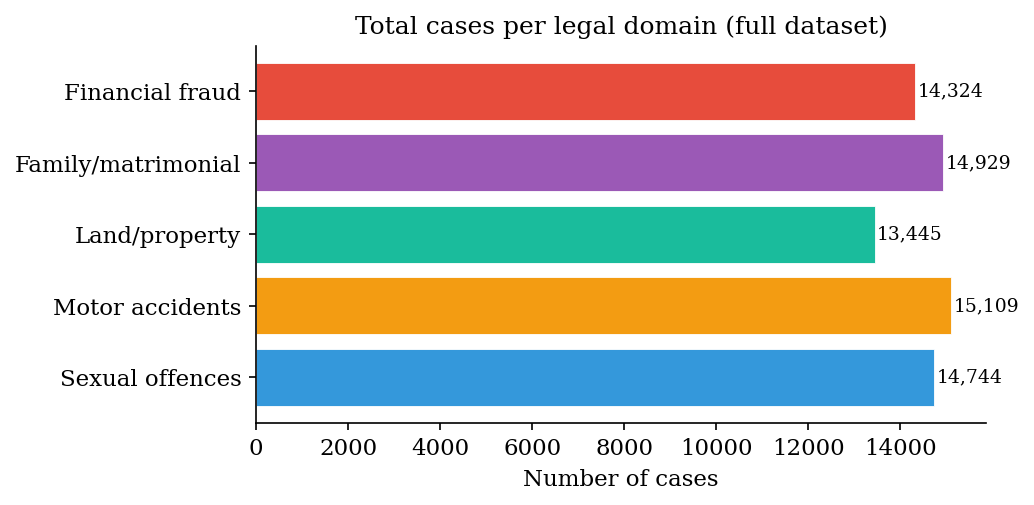
\includegraphics[width=0.92\textwidth]{figures/01_case_counts_full.png}
  \caption{Final case counts per legal domain bucket after multi-hearing merging. All five are within a 10\% range.}
  \label{fig:case_counts}
\end{figure}

Every downstream artefact is produced both per bucket and in a unified \emph{cross-bucket} view, enabling cross-domain transfer and bridge analysis (Chapter~\ref{chap:graph_exploration}).

\section{Named Entity Recognition and Rhetorical Role Classification}
\label{sec:ner_rr}

Before a judgment enters the graph, its raw text is decomposed into typed units: named legal entities anchored to character positions, a rhetorical role for each sentence, and a section-structured summary separating preamble, factual background, arguments, and operative ruling. We use the OpenNyAI legal NLP stack because its NER was trained specifically on Indian judgments (statutory provisions in Indian Parliament style, AIR/SCC citations, party roles such as \textsc{Petitioner}, \textsc{Respondent}, \textsc{Defence Lawyer}), its rhetorical-role classifier reflects Indian High Court discourse conventions, and running it locally on GPU gives reproducible caching as the schema evolves.

\subsection{The OpenNyAI Pipeline}

Three OpenNyAI components run per judgment: \textbf{Legal NER} (\path{en_legal_ner_trf}) with sentence-level inference and post-processing; the \textbf{Rhetorical Role Classifier}, which assigns each sentence one of seven labels (\textsc{Preamble}, \textsc{Facts}, \textsc{Arguments}, \textsc{Ratio}, \textsc{RPC}, \textsc{RLC}, \textsc{None}); and the \textbf{Summarizer}, which produces a four-block summary (\textsc{Preamble}, \textsc{facts}, \textsc{arguments}, \textsc{decision}). The environment is pinned (spaCy~3.2.4, CUDA PyTorch/CuPy) with silent CPU fallback disabled. Each judgment produces one JSON record extended by every subsequent stage.

\subsection{Entity Types and Their Graph Roles}

OpenNyAI recognises twelve entity types; the subset reified as graph nodes is: \textsc{Statute} and \textsc{Provision}; \textsc{Precedent}; \textsc{Court} and \textsc{Judge}; and typed party and counsel roles (\textsc{Petitioner}, \textsc{Respondent}, \textsc{Petitioner\_Lawyer}, \textsc{Defence\_Lawyer}, \textsc{Lawyer}). Auxiliary types (\textsc{Org}, \textsc{GPE}, \textsc{Date}, \textsc{Case\_Number}) are retained in the cleaned JSON but excluded from the final reasoning-focused graph (Section~\ref{sec:graph_schema}).

Entities are canonicalised per bucket: surface forms are normalised (case, whitespace, punctuation) and re-projected as a single \texttt{canonical\_name}. This is what allows the same statute or court to be a \emph{single shared node} across thousands of cases --- the structural property that makes the graph useful for cross-case reasoning.

Figure~\ref{fig:entity_type_totals} confirms that precedents dominate in absolute volume (citation is the primary relational artefact in Indian judgments); party nodes are roughly balanced; statutes and provisions have lower raw counts but carry the most cross-case structural weight, since each canonicalised mention is a potential shared edge. This asymmetry motivates treating statutes, provisions, and precedents as the shared layer while keeping party nodes local to each case.

\begin{figure}[H]
  \centering
  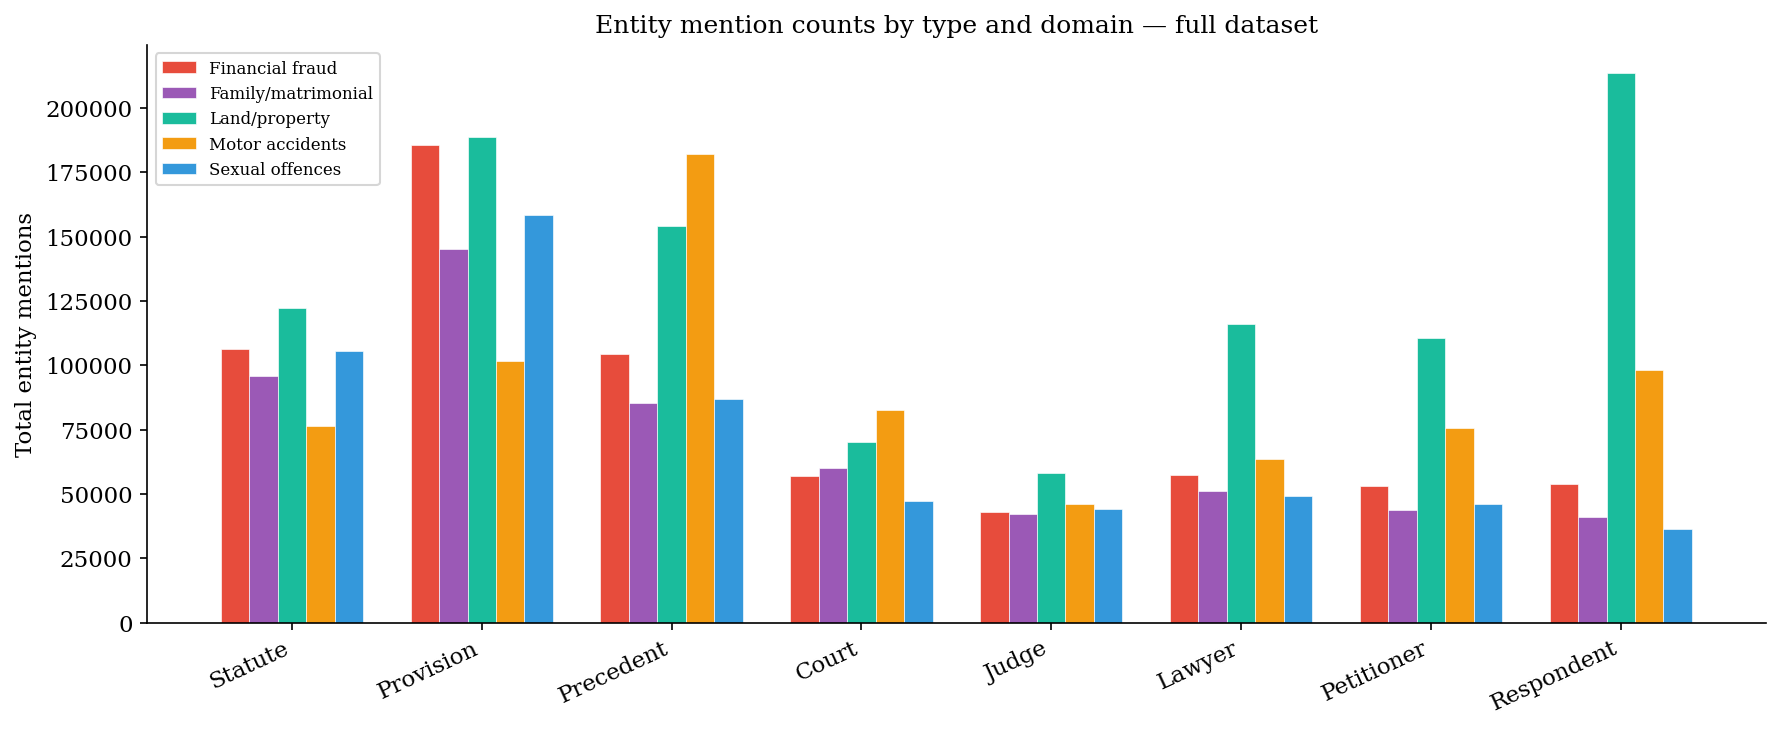
\includegraphics[width=0.92\textwidth]{figures/04_entity_type_totals_full.png}
  \caption{Total entity mention counts by type across the corpus. Precedent mentions dominate; statutes and provisions are smaller but form the shared-node layer.}
  \label{fig:entity_type_totals}
\end{figure}

\subsection{Rhetorical Role Taxonomy and Leakage-Safe Filtering}

Of the seven RR labels, two are inherently decisive: \textbf{RPC} (Ratio and Precedent Cited --- in practice the court's operative paragraph) and \textbf{RLC} (Ruling by Lower Court). Keeping either would let a classifier read the outcome directly. The cleaning stage therefore treats them as forbidden: any annotation whose label intersects \{\textsc{RPC}, \textsc{RLC}\} is dropped, along with any annotation whose summary section is \textsc{decision} or whose label string contains \texttt{"decision"}, \texttt{"disposition"}, \texttt{"operative"}, \texttt{"order"}, or \texttt{"rpc"}. Only the three non-decisive summary fields (\textsc{Preamble}, \textsc{facts}, \textsc{arguments}) are retained as text sources. This is the first leakage gate; a phrase-level gate follows in Section~\ref{sec:leakage_prevention}.

\section{Outcome Labelling with Mistral}
\label{sec:mistral_labelling}

With judgments enriched, we need a case-level outcome label: did the appellant win, lose, or receive a procedural disposition? Labels are produced by prompting a Mistral LLM with the OpenNyAI section-structured summaries. Two properties matter: (i) the labeller sees only the \textsc{decision} block and \textsc{RPC} sentences --- exactly what the leakage-cleaning stage subsequently removes --- so there is no circularity between what is labelled and what the GNN trains on; and (ii) the section-structured input is compact and well-delimited, reducing spurious grounding.

\subsection{Labelling Methodology}

\paragraph{Labels.} Three outcome categories from the perspective of the appellant/petitioner: \texttt{appellant\_won} ($+1$: relief granted, bail allowed, conviction quashed); \texttt{appellant\_lost} ($-1$: dismissed, rejected, bail refused); \texttt{postponed\_or\_procedural} ($0$: adjourned, remanded, liberty granted). Each judgment also carries a \texttt{confidence} rating and a short explanation for auditing.

\paragraph{Cross-validation.} LLM labelling is temperature-sampled, so the same input can yield different labels across runs. To measure this risk, we ran a second independent pass with a fundamentally different prompt: rather than a free-form label, the cross-validation prompt decomposes the task into six directional yes/no questions (three win-signals, three loss-signals) plus a two-question neutrality clause, aggregated deterministically. Concretely, with $S_\text{win}=q_1+q_2+q_3$, $S_\text{loss}=q_4+q_5+q_6$, $S_\text{neutral}=q_7+q_8$: if $S_\text{neutral}>0$, label is \texttt{postponed\_or\_procedural}; otherwise the majority of directional signals wins, ties resolve to procedural, and all-zero responses are excluded as \texttt{unknown}. Because the final label is a deterministic function over binary votes, this pass eliminates free-text generation variance.

\paragraph{Results.} Across 72{,}795 files labelled in both passes, agreement is \textbf{84.4\%} overall (Table~\ref{tab:crossval_agreement}).

\begin{table}[H]
  \centering
  \small
  \begin{adjustbox}{max width=\textwidth}
  \begin{tabular}{lrrr}
    \toprule
    Bucket & Files compared & Matching labels & Agreement rate \\
    \midrule
    Family \& Matrimonial & 15{,}017 & 13{,}049 & 86.9\% \\
    Financial Fraud       & 14{,}342 & 12{,}015 & 83.8\% \\
    Land \& Property      & 13{,}512 &  9{,}652 & 71.4\% \\
    Motor Accidents       & 15{,}117 & 13{,}552 & 89.6\% \\
    Sexual Offences       & 14{,}807 & 13{,}143 & 88.8\% \\
    \midrule
    \textbf{Total}        & \textbf{72{,}795} & \textbf{61{,}411} & \textbf{84.4\%} \\
    \bottomrule
  \end{tabular}
  \end{adjustbox}
  \caption{Cross-run label agreement between the original Mistral pass and the binary-question cross-validation pass.}
  \label{tab:crossval_agreement}
\end{table}

Disagreement is dominated by \textsc{postponed\_or\_procedural} being relabelled as \textsc{appellant\_lost}, most pronounced in Land \& Property where procedural directions (remands, stays) read as adverse to the appellant. The 84\% cross-run agreement establishes that label noise is real but bounded; the ambiguous cases are disproportionately procedural. For the downstream task, \textsc{postponed\_or\_procedural} is excluded from the primary binary task (\texttt{appellant\_won} vs \texttt{appellant\_lost}); agreement on the binary subset is materially higher.

\subsection{Coverage and Label Distribution}

Coverage is near-complete across all five buckets (Figure~\ref{fig:labelling_coverage}); the small unlabelled fraction is malformed JSON or explicit \texttt{unknown} responses, which are excluded. Class distribution (Figures~\ref{fig:outcome_distribution}--\ref{fig:outcome_rate}) is moderately imbalanced: motor-accidents is the most win-skewed, financial-fraud and sexual-offences closest to balanced. The pooled cross-bucket rate of roughly $60\%$ win to $40\%$ loss (binary subset) means a constant-win classifier would achieve misleadingly high accuracy while failing systematically on the loss class, which is why Chapter~\ref{chap:results} reports macro-F1 alongside accuracy.

\begin{figure}[H]
  \centering
  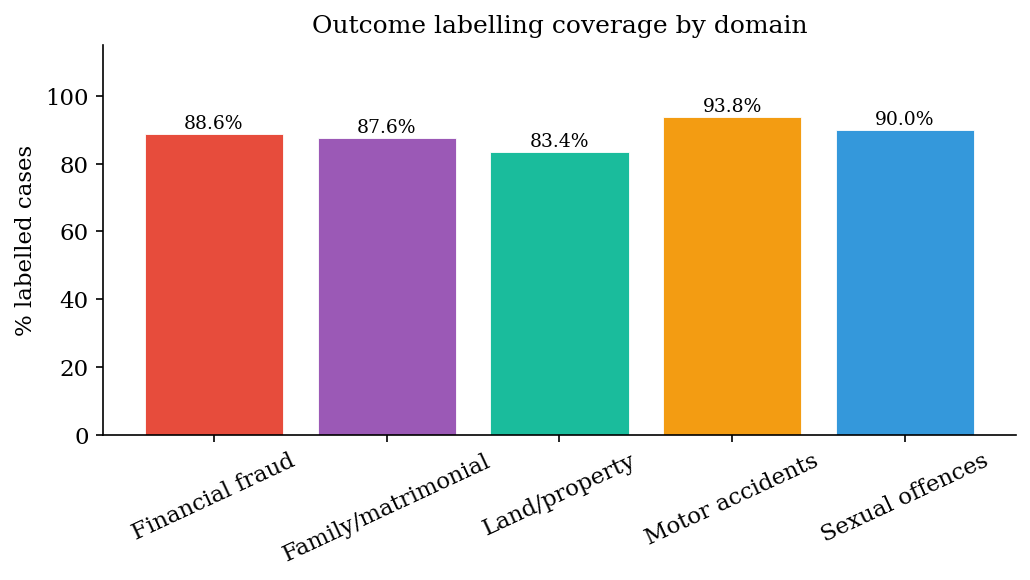
\includegraphics[width=0.92\textwidth]{figures/08_labelling_coverage_full.png}
  \caption{Mistral labelling coverage per bucket.}
  \label{fig:labelling_coverage}
\end{figure}

\begin{figure}[H]
  \centering
  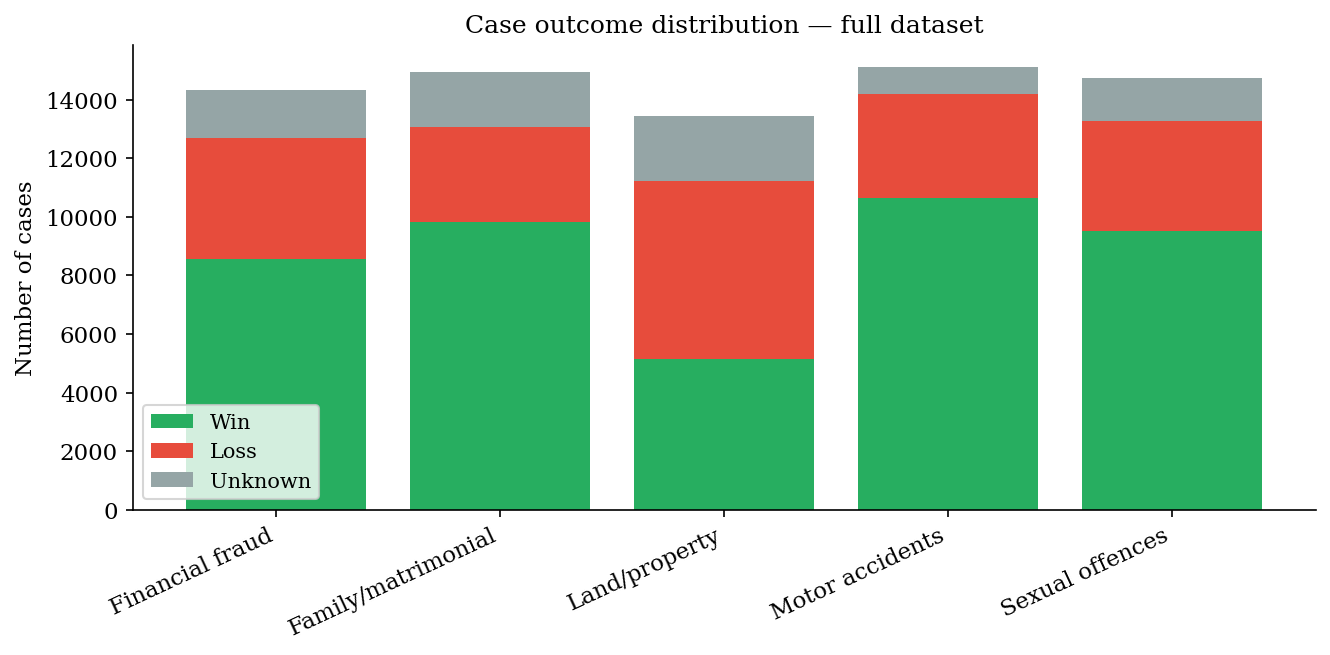
\includegraphics[width=0.92\textwidth]{figures/02_outcome_distribution_full.png}
  \caption{Absolute outcome label counts per bucket.}
  \label{fig:outcome_distribution}
\end{figure}

\begin{figure}[H]
  \centering
  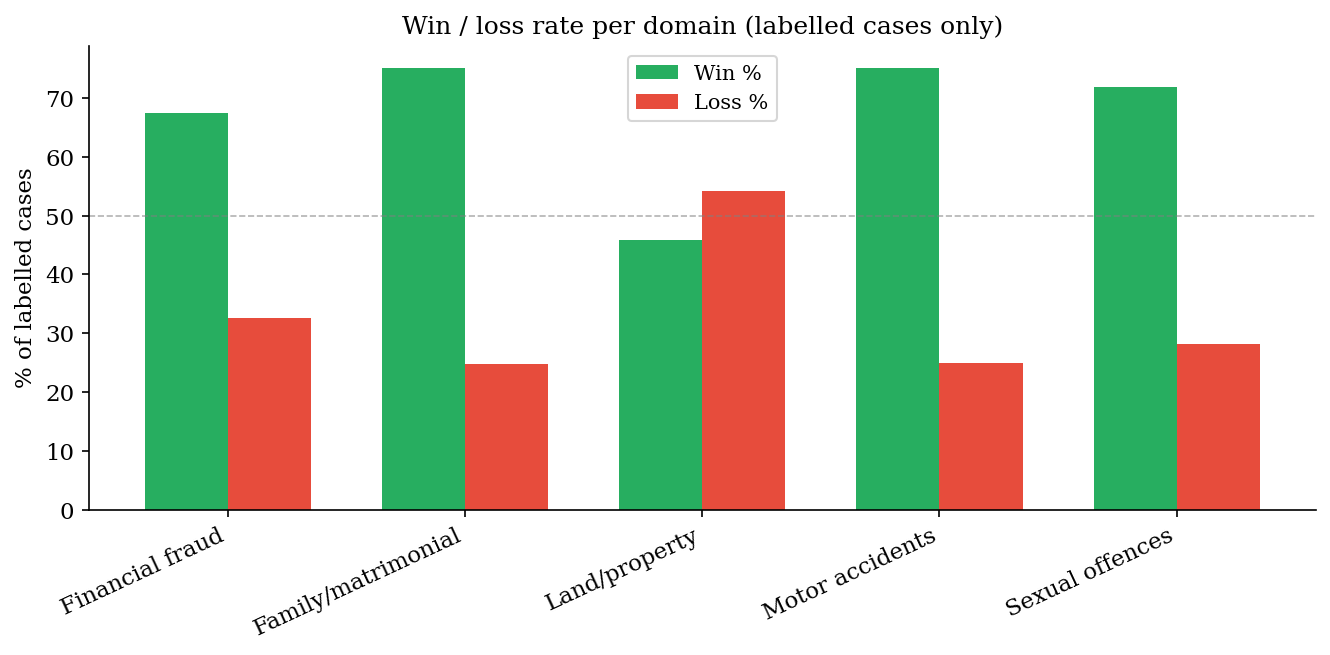
\includegraphics[width=0.92\textwidth]{figures/03_outcome_rate_full.png}
  \caption{Outcome label rates per bucket. Motor-accidents is the most appellant-favourable; financial-fraud and sexual-offences are closest to balanced.}
  \label{fig:outcome_rate}
\end{figure}

\section{Multi-Hearing Merging}
\label{sec:multi_hearing_merging}

A single legal matter frequently produces multiple judgment documents (interim orders, remands, partial disposals, final decision) published as separate PDFs with distinct filenames. If fed in independently, three things go wrong: duplicate \textsc{Case} nodes inflate counts, the final outcome label is not propagated to earlier hearings, and cross-case signals are double-counted.

\paragraph{What counts as the same case.} The merger targets one pattern: a single proceeding heard, adjourned, and returned to the same court on different dates, producing a separate published judgment each time. These are identified by the court-assigned case registration number (e.g., \texttt{5941/2024}, \texttt{Crm-M-44633-2024}), \emph{not} by FIR number --- FIRs identify a police complaint, and one FIR can yield multiple independent proceedings at different courts.

\paragraph{The v1/v2 flaw and v3 fix.} Early versions grouped by case name alone, which could conflate two unrelated proceedings sharing litigant names. The v3 script groups by \texttt{(case\_name,\ case\_number)}; documents with the same name but different registration numbers remain separate, and documents with no extractable registration number are kept as standalone cases.

\paragraph{Extraction.} A three-tier search restricted to preamble material (so case numbers cited as precedents in body text cannot contaminate): (i) regex over the \texttt{PREAMBLE} summary entry; (ii) regex over NER \textsc{Case\_Number} spans in preamble sentences; (iii) regex over the concatenated text of all \textsc{Preamble}-labelled sentences. Seven patterns cover the range of formats in the corpus (\texttt{No.}/\texttt{Nos.}, Punjab/Haryana dash-year, CNR, Delhi~HC \texttt{+}-prefix, and slash-year fallbacks).

\paragraph{Merge mechanics.} Within each group, documents are sorted oldest-to-latest by hearing date. Same-date duplicates are resolved by keeping the file with the most sentences. Multi-date groups have their texts concatenated under labelled dividers (with sentence offsets adjusted), and the final outcome label is always taken from the latest hearing; a containment check suppresses duplicate text regions where the latest document already subsumes an earlier one.

\begin{table}[H]
  \centering
  \small
  \begin{adjustbox}{max width=\textwidth}
  \begin{tabular}{lrrrrr}
    \toprule
    Bucket & Inputs & Final cases & Folded in & Appended & Already contained \\
    \midrule
    Family \& Matrimonial & 15{,}800 & 15{,}306 & 493 & 490 & 3 \\
    Financial Fraud & 15{,}014 & 14{,}615 & 399 & 396 & 3 \\
    Land \& Property & 14{,}324 & 14{,}051 & 251 & 242 & 9 \\
    Motor Accidents & 15{,}271 & 15{,}236 & 32 & 30 & 2 \\
    Sexual Offences & 15{,}532 & 14{,}596 & 936 & 932 & 4 \\
    \midrule
    \textbf{Total} & \textbf{75{,}941} & \textbf{73{,}804} & \textbf{2{,}111}
      & \textbf{2{,}090} & \textbf{21} \\
    \bottomrule
  \end{tabular}
  \end{adjustbox}
  \caption{Multi-hearing merge statistics under the case-number-aware v3 strategy.}
  \label{tab:merge_stats}
\end{table}

Sexual-offences matters fold most aggressively (multiple remand and bail-stage orders); motor-accidents fold least (compensation typically terminates in one tribunal order). Every merge is logged in a per-bucket \texttt{report.json}, making the operation auditable and reversible.

\section{Technology Stack}

The pipeline is Python throughout. OpenNyAI runs on spaCy~3.2.4 with CUDA PyTorch and CuPy in the pinned environment \texttt{fixed\_gpu\_opennyai\_final}. Outcome labelling uses a Mistral model via a batched client. Graph construction uses \texttt{torch\_geometric}'s \texttt{HeteroData}, with text embeddings from \path{BAAI/bge-m3} running multi-process on GPU and cached per bucket. Training, ablation, and analysis scripts live under \path{section_GNN}.
